\documentclass[10pt, a4paper, landscape]{article}

% ----- packages -----
\usepackage{amsmath} % AMS mathematical facilities for LaTeX
\usepackage{enumitem} % Control layout of itemize, enumerate, description
\usepackage{fancyhdr} % Extensive control of page headers and footers in LaTeX2
\usepackage{geometry} % Flexible and complete interface to document dimensions
\usepackage{graphicx} % Enhanced support for graphics
\usepackage{hyperref} % Extensive support for hypertext in LaTeX
\usepackage{multicol} % Intermix single and multiple columns
\usepackage{parskip} % Layout with zero \parindent, non-zero \parskip
\usepackage{tikz} % Create PostScript and PDF graphics in TeX
\usepackage{titlesec} % Select alternative section titles

% ----- random seed -----
\pgfmathsetseed{12}

% ----- custom commands -----
\newcommand{\E}{\mathrm{E}}
\newcommand{\Var}{\mathrm{Var}}
\newcommand{\se}{\mathrm{ee}}
\newcommand{\Cov}{\mathrm{Cov}}
\newcommand{\Corr}{\mathrm{Corr}}
\newcommand{\SSR}{\mathrm{SRC}}
\newcommand{\SSE}{\mathrm{SEC}}
\newcommand{\SST}{\mathrm{STC}}
\newcommand{\tr}{\mathsf{T}}

% ----- page customization -----
\geometry{margin=1cm} % margins config
\pagenumbering{gobble} % remove page numeration
\setlength{\parskip}{0cm} % paragraph spacing
% title spacing
\titlespacing{\section}{0pt}{2ex}{1ex}
\titlespacing{\subsection}{0pt}{1ex}{0ex}
\titlespacing{\subsubsection}{0pt}{0.5ex}{0ex}

% ----- footer -----
\pagestyle{fancy}
\renewcommand{\headrulewidth}{0pt}
\cfoot{\href{https://github.com/marcelomijas/econometrics-cheatsheet}{\normalfont \footnotesize CS-24.5.1-ES - github.com/marcelomijas/econometrics-cheatsheet - CC-BY-4.0 license}}
\setlength{\footskip}{12pt}

% ----- document -----
\begin{document}
	\begin{multicols}{3}
		\begin{center}
			\textbf{\LARGE \href{https://github.com/marcelomijas/econometrics-cheatsheet}{Cheat Sheet Econometría}}
			
			{\footnotesize Por Marcelo Moreno - Universidad Rey Juan Carlos}
			
			{\footnotesize The Econometrics Cheat Sheet Project}
		\end{center}
		
		\section*{Conceptos básicos}
		
		\subsection*{Definiciones}
		
		\textbf{Econometría} - es una disciplina de las ciencias sociales que tiene como objetivo cuantificar las relaciones entre agentes económicos, contrastar teorías económicas y evaluar e implementar políticas públicas y privadas.
		
		\textbf{Modelo econométrico} - es una representación simplificada de la realidad para explicar fenómenos económicos.
		
		\textbf{\textsl{Ceteris paribus}} - si todos los demás factores relevantes permanecen constantes.
		
		\subsection*{Tipos de datos}
		
		\textbf{Sección cruzada} - datos recogidos en un momento dado en el tiempo, una \textsl{foto} estática. El orden no importa.
		
		\textbf{Series temporales} - observación de una/muchas variable/s durante un periodo de tiempo. El orden sí importa.
		
		\textbf{Datos de panel} - consiste una una serie temporal por cada observación de una sección cruzada.
		
		\textbf{Secciones transversales agrupadas} - combina secciones cruzadas de diferentes periodos temporales.
		
		\subsection*{Fases de un modelo econométrico}
		
		\begin{enumerate}[leftmargin=*]
			\setlength{\multicolsep}{0pt}
			\begin{multicols}{2}
				\item Especificación.
				\item Estimación.
				
				\columnbreak
				
				\item Validación.
				\item Utilización.
			\end{multicols}
		\end{enumerate}
		
		\subsection*{Análisis de regresión}
		
		Estudiar y predecir el valor medio de una variable (dependiente, $y$) respecto a unos valores fijos de otras variables (variables independientes, $x$'s). En econometría es común usar Mínimos Cuadrados Ordinarios (MCO) para análisis de regresión.
		
		\subsection*{Análisis de correlación}
		
		El análisis de correlación no distingue entre variables dependientes e independientes.
		
		\begin{itemize}[leftmargin=*]
			\item La correlación simple mide el grado de asociación lineal entre dos variables.
			
			\begin{center}
				$r = \frac{\Cov(x, y)}{\sigma_{x} \cdot \sigma_{y}} = \frac{\sum_{i=1}^{n} ((x_{i} - \overline{x}) \cdot (y_{i} - \overline{y}))}{\sqrt{\sum_{i=1}^{n} (x_{i} - \overline{x})^{2} \cdot \sum_{i=1}^{n} (y_{i} - \overline{y})^{2}}}$
			\end{center}
			
			\item La correlación parcial mide el grado de de asociación lineal entre dos variables controlando una tercera.
		\end{itemize}
		
		\columnbreak
		
		\section*{Supuestos y propiedades}
		
		\subsection*{Supuestos del modelo econométrico}
		
		Bajo estos supuestos, el estimador de MCO presentará buenas propiedades. Supuestos \textbf{Gauss-Markov}:
		
		\begin{enumerate}[leftmargin=*]
			\item \textbf{Linealidad en parámetros} (y dependencia débil en series temporales). $y$ debe ser una función lineal de $\beta$'s.
			\item \textbf{Muestreo aleatorio}. La muestra de la población se ha tomado de forma aleatoria. (Sólo sección cruzada)
			\item \textbf{No colinealidad perfecta}.
			
			\begin{itemize}[leftmargin=*]
				\item No hay variables independientes que sean constantes: $\Var(x_{j}) \neq 0, \; \forall j = 1, \ldots, k$
				\item No hay una relación lineal exacta entre variables independientes.
			\end{itemize}
			
			\item \textbf{Media condicional cero y correlación cero}.
			
			\begin{enumerate}[leftmargin=*, label=\alph{*}.]
				\item No hay errores sistemáticos: $\E(u \mid x_{1}, \ldots, x_{k}) = \E(u) = 0 \rightarrow$ \textbf{exogeneidad fuerte} (a implica b).
				\item No hay variables relevantes fuera del modelo: $\Cov(x_{j}, u) = 0, \; \forall j = 1, \ldots, k \rightarrow$ \textbf{exogeneidad débil}.
			\end{enumerate}
			
			\item \textbf{Homocedasticidad}. La variabilidad de los residuos es igual para todos los niveles de $x$:
			
			$\Var(u \mid x_{1}, \ldots, x_{k}) = \sigma^{2}_{u}$
			
			\item \textbf{No autocorrelación}. Los residuos no contienen información sobre otros residuos:
			
			$\Corr(u_{t}, u_{s} \mid x_{1}, \ldots, x_{k}) = 0, \; \forall t \neq s$
			
			\item \textbf{Normalidad}. Los residuos son independientes e idénticamente distribuidos: $u \sim \mathcal{N}(0, \sigma^{2}_{u})$
			\item \textbf{Tamaño de datos}. El número de observaciones disponibles debe ser mayor a $(k + 1)$ parámetros a estimar. (Ya satisfecho bajo situaciones asintóticas)
		\end{enumerate}
		
		\subsection*{Propiedades asintóticas de MCO}
		
		Bajo los supuestos del modelo econométrico y el Teorema Central del Límite (TCL):
		
		\begin{itemize}[leftmargin=*]
			\item De 1 a 4a: MCO es \textbf{insesgado}. $\E(\hat{\beta}_{j}) = \beta_{j}$
			\item De 1 a 4: MCO es \textbf{consistente}. $\mathrm{plim}(\hat{\beta}_{j}) = \beta_{j}$ (a 4b sin 4a, exogeneidad	débil, insesgado y consistente).
			\item De 1 a 5: \textbf{normalidad asintótica} de MCO (entonces, 7 es necesariamente satisfecho): $u \underset{a}{\sim}\mathcal{N}(0, \sigma^{2}_{u})$
			\item De 1 a 6: \textbf{estimador insesgado} de $\sigma^{2}_{u}$. $\E(\hat{\sigma}^{2}_{u}) = \sigma^{2}_{u}$
			\item De 1 a 6: MCO es MELI (Mejor Estimador Lineal Insesgado, \textcolor{blue}{BLUE} en inglés) ó \textbf{eficiente}.
			\item De 1 a 7: contrastes de hipótesis e intervalos de confianza son fiables.
		\end{itemize}
		
		\columnbreak
		
		\section*{Mínimos Cuadrados Ordinarios}
		
		\textbf{Objetivo} - minimizar Suma de Resid. Cuadrados (SRC):
		
		\begin{center}
			$\min \sum_{i=1}^{n} \hat{u}^{2}_{i}$, donde $\hat{u}_{i} = y_{i} - \hat{y}_{i}$
		\end{center}
		
		\subsection*{Modelo de regresión simple}
		
		\setlength{\multicolsep}{2pt}
		\setlength{\columnsep}{-40pt}
		\begin{multicols}{2}
			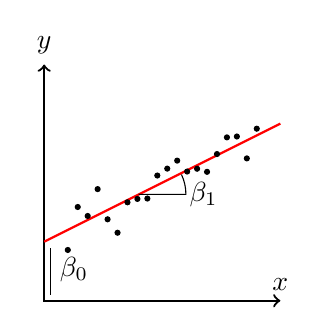
\begin{tikzpicture}[scale=0.15]
				% \draw [step=1, gray, very thin] (0, 0) grid (20, 20);
				\draw [thick, <->] (0, 20) node [anchor=south] {$y$} -- (0, 0) -- (20, 0) node [anchor=south] {$x$}; 
				\draw [red, thick] plot [domain=0:20] (\x, {5 + 0.5*\x});
				\draw plot [only marks, mark=*, mark size=6, domain=2:18, samples=20] (\x, {rnd*5 + 2.5 + 0.5*\x}); 
				\draw (0.5, 0.5) -- (0.5, 4.5) node [anchor=north west] {$\beta_{0}$}; 
				\draw (8, 9) -- (12, 9) arc (0:25:4); 
				\draw (13.5, 9) node {$\beta_{1}$};
			\end{tikzpicture}
			
			\columnbreak
			
			Ecuación:
			
			\begin{center}
				$y_{i} = \beta_{0} + \beta_{1} x_{i} + u_{i}$
			\end{center}
			
			Estimación:
			
			\begin{center}
				$\hat{y}_{i} = \hat{\beta}_{0} + \hat{\beta}_{1} x_{i}$
			\end{center}
			
			donde:
			
			\begin{center}
				$\hat{\beta}_{0} = \overline{y} - \hat{\beta}_{1} \overline{x}$
				
				$\hat{\beta}_{1} = \frac{\Cov(y, x)}{\Var(x)}$
			\end{center}
		\end{multicols}
		
		\subsection*{Modelo de regresión múltiple}
		
		\setlength{\multicolsep}{2pt}
		\setlength{\columnsep}{-40pt}
		\begin{multicols}{2}
			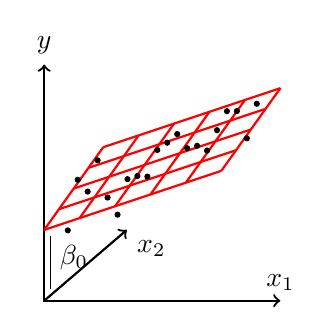
\begin{tikzpicture}[scale=0.15]
				% \draw [step=1, gray, very thin] (0, 0) grid (20, 20);
				\draw [thick, ->] (0, 0) -- (7, 6) node [anchor=north west] {$x_{2}$}; 
				\draw [thick, <->] (0, 20) node [anchor=south] {$y$} -- (0, 0) -- (20, 0) node [anchor=south] {$x_{1}$}; 
				\draw [red, thick] (0, 6) -- (5, 13); 
				\draw [red, thick] (3, 7) -- (8, 14); 
				\draw [red, thick] (6, 8) -- (11, 15); 
				\draw [red, thick] (9, 9) -- (14, 16); 
				\draw [red, thick] (12, 10) -- (17, 17); 
				\draw [red, thick] (15, 11) -- (20, 18); 
				\draw [red, thick] (0, 6) -- (15, 11);
				\draw [red, thick] (1.25, 7.75) -- (16.25, 12.75); 
				\draw [red, thick] (2.5, 9.5) -- (17.5, 14.5); 
				\draw [red, thick] (3.75, 11.25) -- (18.75, 16.25);
				\draw [red, thick] (5, 13) -- (20, 18); 
				\draw plot [only marks, mark=*, mark size=6, domain=2:18, samples=20] (\x, {rnd*6 + 4 + 0.5*\x}); 
				\draw (0.5, 1) -- (0.5, 5.5) node [anchor=north west] {$\beta_{0}$};
			\end{tikzpicture}
			
			\columnbreak
			
			Ecuación:
			
			\begin{center}
				$y_{i} = \beta_{0} + \beta_{1} x_{1i} + \cdots + \beta_{k} x_{ki} + u_{i}$
			\end{center}
			
			Estimación:
			
			\begin{center}
				$\hat{y}_{i} = \hat{\beta}_{0} + \hat{\beta}_{1} x_{1i} + \cdots + \hat{\beta}_{k} x_{ki}$
			\end{center}
			
			donde:
			
			\begin{center}
				$\hat{\beta}_{0} = \overline{y} - \hat{\beta}_{1} \overline{x}_{1} - \cdots - \hat{\beta}_{k} \overline{x}_{k}$
				
				$\hat{\beta}_{j} = \frac{\Cov(y, \text{resid } x_{j})}{\Var(\text{resid } x_{j})}$
			\end{center}
			
			Matriz: $\hat{\beta} = (X^{\tr} X)^{-1}(X^{\tr} y)$
		\end{multicols}
		
		\subsection*{Interpretación de coeficientes}
		
		\begin{center}
			\scalebox{0.85}{
				\begin{tabular}{ c c c c }
					Modelo      & Depend.   & Independ.   & Interpretación $\beta_{1}$                        \\ \hline
					Nivel-nivel & $y$       & $x$         & $\Delta y = \beta_{1} \Delta x$                   \\
					Nivel-log   & $y$       & $\log(x)$   & $\Delta y \approx (\beta_{1}/100) (\% \Delta x$)  \\
					Log-nivel   & $\log(y)$ & $x$         & $\% \Delta y \approx (100 \beta_{1}) \Delta x$    \\
					Log-log     & $\log(y)$ & $\log(x)$   & $\% \Delta y \approx \beta_{1} (\% \Delta x$)     \\
					Cuadrático  & $y$       & $x + x^{2}$ & $\Delta y = (\beta_{1} + 2 \beta_{2} x) \Delta x$
				\end{tabular}
			}
		\end{center}
		
		\subsection*{Medidas de error}
		
		Suma de Resid. Cuad.: \hfill $\SSR = \sum_{i=1}^{n} \hat{u}_{i}^{2} = \sum_{i=1}^{n} (y_{i} - \hat{y}_{i})^{2}$
		
		Suma Explicada de Cuadrados: \hfill $\SSE = \sum_{i=1}^{n} (\hat{y}_{i} - \overline{y})^{2}$
		
		Suma Tot. de Cuad.: \hfill $\SST = \SSE + \SSR = \sum_{i=1}^{n} (y_{i} - \overline{y})^{2}$
		
		Error Estándar de la Regresión: \hfill $\hat{\sigma}_{u} = \sqrt{\frac{\SSR}{n - k - 1}}$
		
		Error Estándar de los $\hat{\beta}$'s: \hfill $\se(\hat{\beta}) = \sqrt{\hat{\sigma}^{2}_{u} \cdot (X^{\tr} X)^{-1}}$
		
		Raíz del Error Cuadrático Medio: \hfill $\mathrm{RECM} = \sqrt{\frac{\sum_{i=1}^{n} (y_{i} - \hat{y}_{i})^{2}}{n}}$
		
		Error Medio Absoluto: \hfill $\mathrm{EMA} = \frac{\sum_{i=1}^{n} \lvert y_{i} - \hat{y}_{i} \rvert}{n}$
		
		Porcentaje Medio de Error: \hfill $\mathrm{PME} = \frac{\sum_{i=1}^{n} \lvert \hat{u}_{i} / y_{i} \rvert}{n} \cdot 100$
		
		\columnbreak
		
		\section*{R-cuadrado}
		
		Es una medida de la \textbf{bondad del ajuste}, cómo la regresión se ajusta a los datos:
		
		\begin{center}
			$R^{2} = \frac{\SSE}{\SST} = 1 - \frac{\SSR}{\SST}$
		\end{center}
		
		\begin{itemize}[leftmargin=*]
			\item Mide el \textbf{porcentaje de variación} en $y$ que es linealmente \textbf{explicado} por variaciones de las $x$'s.
			\item Toma valores \textbf{entre 0} (no hay explicación lineal) \textbf{y 1} (explicación total).
		\end{itemize}
		
		Cuando el número de regresores incrementa, el R-cuadrado también, independientemente de si las nuevas variables son relevantes o no. Para resolver este problema, hay un \textbf{R-cuadrado ajustado} por grados de libertad (o corregido):
		
		\begin{center}
			$\overline{R}^{2} = 1 - \frac{n - 1}{n - k - 1} \cdot \frac{\SSR}{\SST} = 1 - \frac{n - 1}{n - k - 1} \cdot (1 - R^{2})$
		\end{center}
		
		Para muestras grandes: $\overline{R}^{2} \approx R^{2}$
		
		\section*{Contrastes de hipótesis}
		
		\subsection*{Definiciones}
		
		Es una regla diseñada para, a partir de una muestra, explicar si existe \textbf{evidencia para rechazar (o no) una hipótesis} sobre uno o más parámetros poblacionales.
		
		Elementos de un contraste de hipótesis:
		
		\begin{itemize}[leftmargin=*]
			\item \textbf{Hipótesis nula} ($H_{0}$) - es la hipótesis a ser probada.
			\item \textbf{Hipótesis alternativa} ($H_{1}$) - el la hipótesis que no puede rechazarse si $H_{0}$ es rechazada.
			\item \textbf{Estadístico de contraste} - es una variable aleatoria cuya distribución de probabilidad es conocida bajo $H_{0}$.
			\item \textbf{Valor crítico} ($C$) - es el valor contra el cual se compara el estadístico de contraste para determinar si se rechaza o no la hipótesis nula. Determina la frontera entre la región de aceptación y la de rechazo de $H_{0}$.
			\item \textbf{Nivel de significación} ($\alpha$) - es la probabilidad de rechazar la $H_{0}$ siendo cierta (Error Tipo I). Es elegido por quien conduce el contraste. Usualmente 10\%, 5\% ó 1\%.
			\item \textbf{p-valor} - es el nivel de significación máximo por el cual $H_{0}$ no puede ser rechazada.
		\end{itemize}
		
		\setlength{\multicolsep}{0pt}
		\setlength{\columnsep}{20pt}
		\begin{multicols}{2}
			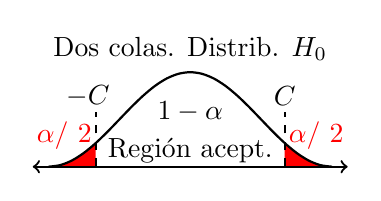
\begin{tikzpicture}[scale=0.10]
				\node at (0, 15) {Dos colas. Distrib. $H_{0}$}; 
				\fill [red] (12, 0) -- plot [domain=12:18, smooth] (\x, {cos(\x*10)*6 + 6}); 
				\fill [red] (-12, 0) -- plot [domain=-18:-12, smooth] (\x, {cos(\x*10)*6 + 6}); 
				\draw [thick] plot [domain=-18:18, smooth] (\x, {cos(\x*10)*6 + 6}); 
				\draw [thick, <->] (-20, 0) -- (20, 0); 
				\draw [thick, dashed] (12, 0) -- (12, 7); 
				\draw [thick, dashed] (-12, 0) -- (-12, 7); 
				\node at (0, 2) {Región acept.}; 
				\node at (0, 7) {$1 - \alpha$}; 
				\node [red] at (-16, 4) {$\alpha /\ 2$}; 
				\node [red] at (16, 4) {$\alpha /\ 2$}; 
				\node at (12, 9) {$C$}; 
				\node at (-13, 9) {$-C$};
			\end{tikzpicture}
			
			\columnbreak
			
			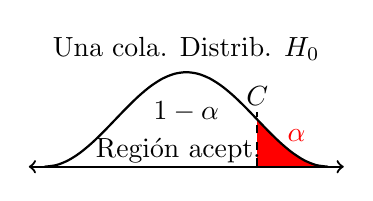
\begin{tikzpicture}[scale=0.10]
				\node at (0, 15) {Una cola. Distrib. $H_{0}$}; 
				\fill [red] (9, 0) -- plot [domain=9:18, smooth] (\x, {cos(\x*10)*6 + 6}); 
				\draw [thick] plot [domain=-18:18, smooth] (\x, {cos(\x*10)*6 + 6}); 
				\draw [thick, <->] (-20, 0) -- (20, 0); 
				\draw [thick, dashed] (9, 0) -- (9, 7); 
				\node at (-1, 2) {Región acept.};
				\node at (0, 7) {$1 - \alpha$}; 
				\node [red] at (14, 4) {$\alpha$}; 
				\node at (9, 9) {$C$};
			\end{tikzpicture}
		\end{multicols}
		
		\textbf{Regla general}: si p-valor $< \alpha$, existe evidencia para rechazar $H_{0}$, es decir, existe evidencia para aceptar $H_{1}$.
		
		\columnbreak
		
		\subsection*{Contrastes individuales}
		
		Prueba si un parámetro es significativamente diferente de un cierto valor, $\vartheta$.
		
		\begin{itemize}[leftmargin=*]
			\item $H_{0}: \beta_{j} = \vartheta$
			\item $H_{1}: \beta_{j} \neq \vartheta$
		\end{itemize}
		
		\begin{center}
			Bajo $H_{0}$: \quad $t = \frac{\hat{\beta}_{j} - \vartheta}{\se(\hat{\beta}_{j})} \sim t_{n - k - 1, \alpha/2}$
		\end{center}
		
		Si $\lvert t \rvert > \lvert t_{n - k - 1, \alpha/2} \rvert$, existe evidencia para rechazar $H_{0}$.
		
		\textbf{Contraste de significación individual} - prueba si un parámetro es \textbf{significativamente distinto de cero}.
		
		\begin{itemize}[leftmargin=*]
			\item $H_{0}: \beta_{j} = 0$
			\item $H_{1}: \beta_{j} \neq 0$
		\end{itemize}
		
		\begin{center}
			Bajo $H_{0}$: \quad $t = \frac{\hat{\beta}_{j}}{\se(\hat{\beta}_{j})}\sim t_{n - k - 1, \alpha/2}$
		\end{center}
		
		Si $\lvert t \rvert > \lvert t_{n - k - 1, \alpha/2} \rvert$, existe evidencia para rechazar $H_{0}$.
		
		\subsection*{Contraste F}
		
		Prueba simultáneamente múltiples hipótesis (lineales) sobre los parámetros. Hace uso de un modelo no restringido y uno restringido:
		
		\begin{itemize}[leftmargin=*]
			\item \textbf{Modelo no restringido} - es el modelo donde se quiere probar la hipótesis.
			\item \textbf{Modelo restringido} - es el modelo donde se ha impuesto la hipótesis que se quiere probar.
		\end{itemize}
		
		Entonces, viendo los errores, hay:
		
		\begin{itemize}[leftmargin=*]
			\item \textbf{$\SSR_{\mathrm{UR}}$} - es la $\SSR$ del modelo no restringido.
			\item \textbf{$\SSR_{\mathrm{R}}$} - es la $\SSR$ del modelo restringido.
		\end{itemize}
		
		\begin{center}
			Bajo $H_{0}$: \quad $F = \frac{\SSR_{\mathrm{R}}- \SSR_{\mathrm{UR}}}{\SSR_{\mathrm{UR}}} \cdot \frac{n - k - 1}{q} \sim F_{q, n - k - 1}$
		\end{center}
		
		donde $k$ es el número de parámetros del modelo no restringido y $q$ es el número de hipótesis lineales a probar.
		
		Si $F > F_{q, n - k - 1}$, existe evidencia para rechazar $H_{0}$.
		
		\textbf{Contraste de significación global} - prueba si todos los parametros asociados a $x$'s son \textbf{simultáneamente cero}.
		
		\begin{itemize}[leftmargin=*]
			\item $H_{0}: \beta_{1} = \beta_{2} = \cdots = \beta_{k} = 0$
			\item $H_{1}: \beta_{1} \neq 0$ y/o $\beta_{2} \neq 0 \ldots$ y/o $\beta_{k} \neq 0$
		\end{itemize}
		
		Podemos simplificar la fórmula para el estadístico $F$:
		
		\begin{center}
			Bajo $H_{0}$: \quad $F = \frac{R^{2}}{1 - R^{2}} \cdot \frac{n - k - 1}{k} \sim F_{k, n - k - 1}$
		\end{center}
		
		Si $F > F_{k, n - k - 1}$, existe evidencia para rechazar $H_{0}$.
		
		\section*{Intervalos de confianza}
		
		Los intervalos de confianza al nivel de confianza ($1 - \alpha$), se pueden calcular:
		
		\begin{center}
			$\hat{\beta}_{j} \mp t_{n - k - 1, \alpha/2} \cdot \se(\hat{\beta}_{j})$
		\end{center}
		
		\columnbreak
		
		\section*{Variables ficticias}
		
		Las variables ficticias (o binarias) son usadas para recoger información cualitativa: sexo, estado civil, país, etc.
		
		\begin{itemize}[leftmargin=*]
			\item Toman \textbf{valor 1} en una categoría dada y \textbf{0 en el resto}.
			\item Se usan para analizar y modelizar \textbf{cambios estructurales} en los parámetros del modelo.
		\end{itemize}
		
		Si una variable cualitativa tiene $m$ categorías, sólo hay que incluir ($m - 1$) variables ficticias en el modelo.
		
		\subsection*{Cambio estructural}
		
		El cambio estructural se refiere a los cambios en los valores de los parámetros del modelo producidos por el efecto de diferentes sub-poblaciones. El cambio estructural se puede incluir en el modelo a través de variables ficticias.
		
		La ubicación de las variables ficticias ($D$) es importante:
		
		\begin{itemize}[leftmargin=*]
			\item \textbf{En la constante} (efecto aditivo) - representa la diferencia media entre los valores producidos por el cambio estructural.
			
			\begin{center}
				$y = \beta_{0} + \delta_{1} D + \beta_{1} x_{1} + u$
			\end{center}
			
			\item \textbf{En la pendiente} (efecto multiplicativo) - representa la diferencia en el efecto (pendiente) entre los valores producidos por el cambio estructural.
			
			\begin{center}
				$y = \beta_{0} + \beta_{1} x_{1} + \delta_{1} D \cdot x_{1} + u$
			\end{center}
		\end{itemize}
		
		\textbf{Contraste de Chow para cambio estructural} - analiza la existencia de cambio estructural en todos los parámetros del modelo, es una expresión particular del contraste F, donde $H_{0}$: No hay cambio estructural (todos $\delta = 0$).
		
		\section*{Cambios de escala}
		
		Cambios en las \textbf{unidades de medida} de las variables:
		
		\begin{itemize}[leftmargin=*]
			\item Sobre la variable \textbf{endógena}, $y^{*} = y \cdot \lambda$ - afecta a todos los parámetros del modelo, $\beta_{j}^{*} = \beta_{j} \cdot \lambda, \; \forall j = 1, \ldots, k$
			\item Sobre una variable \textbf{exógena}, $x_{j}^{*} = x_{j} \cdot \lambda$ - sólo afecta al parámetro ligado a dicha variable exógena, $\beta_{j}^{*} = \beta_{j} \cdot \lambda$
			\item Mismo cambio de escala sobre endógena y exógena - sólo afecta al término constante, $\beta_{0}^{*} = \beta_{0} \cdot \lambda$
		\end{itemize}
		
		\section*{Cambios de origen}
		
		Cambios en el \textbf{origen de medida} de las variables (endógenas o exógenas), $y^{*} = y + \lambda$ - sólo afectan al término constante del modelo, $\beta_{0}^{*} = \beta_{0} + \lambda$
		
		\columnbreak
		
		\section*{Multicolinealidad}
		
		\begin{itemize}[leftmargin=*]
			\item \textbf{Multicolinealidad perfecta} - hay variables independientes que son constantes y/o hay una relación lineal exacta entre variables independientes. Es el \textbf{incumplimiento del tercer (3) supuesto} del modelo.
			\item \textbf{Multicolinealidad aproximada} - hay variables independientes que son aproximadamente constantes y/o hay una relación lineal aproximada entre variables independientes. \textbf{No implica el incumplimiento de algún supuesto} del modelo, pero tiene un efecto en MCO.
		\end{itemize}
		
		\subsection*{Consecuencias}
		
		\begin{itemize}[leftmargin=*]
			\item \textbf{Multicolinealidad perfecta} - el sistema de ecuaciones de MCO no puede resolverse (infinitas soluciones).
			\item \textbf{Multicolinealidad aproximada}
			
			\begin{itemize}[leftmargin=*]
				\item Pequeñas variaciones en la muestra producen grandes variaciones en las estimaciones de MCO.
				\item La varianza de los estimadores MCO de las $x$'s que son colineales incrementa, la inferencia de los parámetros es afectada (intervalo de confianza grande).
			\end{itemize}
		\end{itemize}
		
		\subsection*{Detección}
		
		\begin{itemize}[leftmargin=*]
			\item \textbf{Análisis de correlación} - buscar altas correlaciones entre variables independientes, $\lvert r \rvert > 0.7$.
			\item \textbf{Factor de Inflación de la Varianza (FIV o VIF)} - indica el incremento en $\Var(\hat{\beta}_{j})$ debido a la multicolinealidad.
			
			\begin{center}
				$\mathrm{VIF}(\hat{\beta}_{j}) = \frac{1}{1 - R_{j}^{2}}$
			\end{center}
			
			donde $R^{2}_{j}$ denota el R-cuadrado de una regresión entre $x_{j}$ y todas las otras $x$'s.
			
			\begin{itemize}[leftmargin=*]
				\item Valores entre 4 y 10 - pueden existir problemas de multicolinealidad.
				\item Valores $>$ 10 - existen problemas de multicolinealidad.
			\end{itemize}
		\end{itemize}
		
		Una característica típica de la multicolinealidad es que los coeficientes de regresión del modelo no son individualmente significativos (por las altas varianzas), pero sí que son conjuntamente significativos.
		
		\subsection*{Corrección}
		
		\begin{itemize}[leftmargin=*]
			\item Eliminar una de las variables colineales.
			\item Realizar análisis factorial(u otra técnica de reducción de dimensiones) en las vairables colineales.
			\item Interpretar los coeficientes con multicolinealidad conjuntamente.
		\end{itemize}
		
		\columnbreak
		
		\section*{Heterocedasticidad}
		
		Los residuos $u_{i}$ de la función de regresión poblacional no tienen una varianza constante $\sigma^{2}_{u}$:
		
		\begin{center}
			$\Var(u \mid x_{1}, \ldots, x_{k}) = \Var(u) \neq \sigma^{2}_{u}$
		\end{center}
		
		Es el \textbf{incumplimiento del quinto (5) supuesto} del modelo.
		
		\subsection*{Consecuencias}
		
		\begin{itemize}[leftmargin=*]
			\item Estimadores MCO son insesgados.
			\item Estimadores MCO son consistentes.
			\item MCO ya \textbf{no es eficiente}, pero sigue siendo ELI (Estimador Lineal Insesgado).
			\item La \textbf{estimación de la varianza} de los estimadores es \textbf{sesgada}: la construcción de intervalos de confianza y contraste de hipótesis no son fiables.
		\end{itemize}
		
		\subsection*{Detección}
		
		\begin{itemize}[leftmargin=*]
			\setlength{\multicolsep}{0pt}
			\setlength{\columnsep}{20pt}
			\begin{multicols}{3}
				\item \textbf{Gráficos} - buscar patrones de dispersión en gráficos $x$ vs. $u$ ó $x$ vs. $y$.
				
				\columnbreak
				
				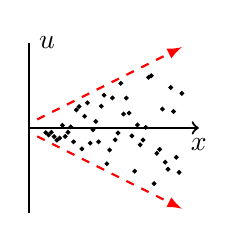
\begin{tikzpicture}[scale=0.108]
					% \draw [step=1, gray, very thin] (0, 0) grid (20, 20);
					\draw [thick, ->] (0, 10) -- (20, 10) node [anchor=north] {$x$}; 
					\draw [thick, -] (0, 0) -- (0, 20) node [anchor=west] {$u$}; 
					\draw plot [only marks, mark=*, mark size=6, domain=2:18, samples=50] (\x, {-0.5*rand*\x + 10}); 
					\draw [thick, dashed, red, -latex] plot [domain=1:18] (\x, {-0.5*\x + 9.5}); 
					\draw [thick, dashed, red, -latex] plot [domain=1:18] (\x, {0.5*\x + 10.5});
				\end{tikzpicture}
				
				\columnbreak
				
				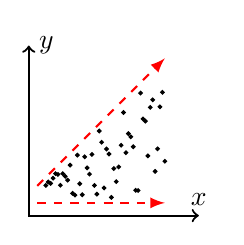
\begin{tikzpicture}[scale=0.108]
					% \draw [step=1, gray, very thin] (0, 0) grid (20, 20);
					\draw [thick, <->] (0, 20) node [anchor=west] {$y$} -- (0, 0) -- (20, 0) node [anchor=south] {$x$}; 
					\draw plot [only marks, mark=*, mark size=6, domain=2:16, samples=50] (\x, {0.5*\x*(rand + 1) + 2}); 
					\draw [thick, dashed, red, -latex] plot [domain=1:16] (\x, {1.5}); 
					\draw [thick, dashed, red, -latex] plot [domain=1:16] (\x, {1*\x + 2.5});
				\end{tikzpicture}
			\end{multicols}
			
			\item \textbf{Test formales} - White, Bartlett, Breusch-Pagan, etc. Comúnmente, $H_{0}$: No heterocedasticidad.
		\end{itemize}
		
		\subsection*{Corrección}
		
		\begin{itemize}[leftmargin=*]
			\item Usar MCO con un estimador de la matriz de varianzas-covarianzas robusto a la heterocedasticidad (HC), por ejemplo, la propuesta de White.
			\item Si la estructura de la varianza es conocida, usar Mínimos Cuadrados Ponderados (MCP) o Mínimos Cuadrados Generalizados (MCG):
			
			\begin{itemize}[leftmargin=*]
				\item Suponiendo que $\Var(u) = \sigma^{2}_{u} \cdot x_{i}$, dividir las variables del modelo entre la raíz cuadrada de $x_{i}$ y aplicar MCO.
				\item Suponiendo que $\Var(u) = \sigma^{2}_{u} \cdot x_{i}^{2}$, dividir las variables del modelo entre $x_{i}$ (la raíz cuadrada de $x_{i}^{2}$) y aplicar MCO.
			\end{itemize}
			
			\item Si la estructura de la varianza es desconocida, hacer uso de Mínimos Curadrados Ponderados Factibles (MCPF), que estima una posible varianza, divide las variables del modelo entre ella y entonces aplica MCO.
			\item Nueva especificación del modelo, por ejemplo, transformación logarítmica (reduce la varianza).
		\end{itemize}
		
		\columnbreak
		
		\section*{Autocorrelación}
		
		El residuo de cualquier observación, $u_{t}$, está correlacionado con el residuo de cualquier otra observación. Las observaciones no son independientes.
		
		\begin{center}
			$\Corr(u_{t}, u_{s} \mid x_{1}, \ldots, x_{k}) = \Corr(u_{t}, u_{s}) \neq 0, \quad \forall t \neq s$
		\end{center}
		
		El contexto ``natural" de este fenómeno son las series temporales. Es el \textbf{incumplimiento del sexto (6) supuesto} del modelo.
		
		\subsection*{Consecuencias}
		
		\begin{itemize}[leftmargin=*]
			\item Estimadores MCO son insesgados.
			\item Estimadores MCO son consistentes.
			\item MCO ya \textbf{no es eficiente}, pero sigue siendo ELI (Estimador Lineal Insesgado).
			\item La \textbf{estimación de la varianza} de los estimadores es \textbf{sesgada}: la construcción de intervalos de confianza y contraste de hipótesis no son fiables.
		\end{itemize}
		
		\subsection*{Detección}
		
		\begin{itemize}[leftmargin=*]
			\item \textbf{Gráficos} - buscar patrones de dispersión en gráficos $u_{t - 1}$ vs. $u_{t}$ o hacer uso del correlograma.
			
			\setlength{\multicolsep}{0pt}
			\setlength{\columnsep}{6pt}
			\begin{multicols}{3}
				\begin{center}
					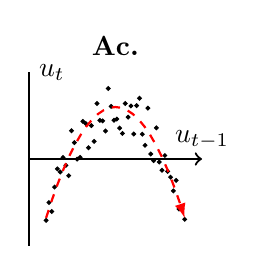
\begin{tikzpicture}[scale=0.11]
						% \draw [step=1, gray, very thin] (0, 0) grid (20, 23);
						\node at (10, 23) {\textbf{Ac.}}; 
						\draw [thick, ->] (0, 10) -- (20, 10) node [anchor=south] {$u_{t - 1}$}; 
						\draw [thick, -] (0, 0) -- (0, 20) node [anchor=west] {$u_{t}$}; 
						\draw plot [only marks, mark=*, mark size=6, domain=2:18, samples=50] (\x, {-0.2*(\x - 10)^2 + 13 + 6*rnd}); 
						\draw [thick, dashed, red, -latex] plot [domain=2:18] (\x, {-0.2*(\x - 10)^2 + 16});
					\end{tikzpicture}
				\end{center}
				
				\columnbreak
				
				\begin{center}
					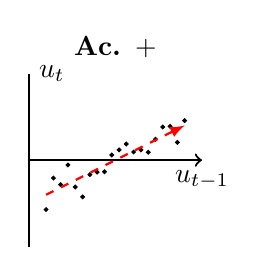
\begin{tikzpicture}[scale=0.11]
						% \draw [step=1, gray, very thin] (0, 0) grid (20, 23);
						\node at (10, 23) {\textbf{Ac. $+$}}; 
						\draw [thick, ->] (0, 10) -- (20, 10) node [anchor=north] {$u_{t - 1}$}; 
						\draw [thick, -] (0, 0) -- (0, 20) node [anchor=west] {$u_{t}$}; 
						\draw plot [only marks, mark=*, mark size=6, domain=2:18, samples=20] (\x, {5*rnd + 2.5 + 0.5*\x}); 
						\draw [thick, dashed, red, -latex] plot [domain=2:18] (\x, {5 + 0.5*\x});
					\end{tikzpicture}
				\end{center}
				
				\columnbreak
				
				\begin{center}
					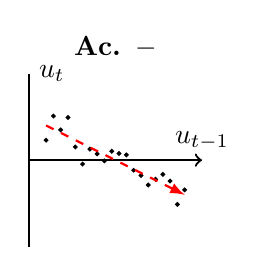
\begin{tikzpicture}[scale=0.11]
						% \draw [step=1, gray, very thin] (0, 0) grid (20, 23);
						\node at (10, 23) {\textbf{Ac. $-$}}; 
						\draw [thick, ->] (0, 10) -- (20, 10) node [anchor=south] {$u_{t - 1}$}; 
						\draw [thick, -] (0, 0) -- (0, 20) node [anchor=west] {$u_{t}$}; 
						\draw plot [only marks, mark=*, mark size=6, domain=2:18, samples=20] (\x, {5*rnd + 12.5 - 0.5*\x}); 
						\draw [thick, dashed, red, -latex] plot [domain=2:18] (\x, {15 - 0.5*\x});
					\end{tikzpicture}
				\end{center}
			\end{multicols}
			
			\item \textbf{Test formales} - Durbin-Watson, Breusch-Godfrey, etc. Comúnmente, $H_{0}$: No autocorrelación.
		\end{itemize}
		
		\subsection*{Corrección}
		
		\begin{itemize}[leftmargin=*]
			\item Usar MCO con un estimador de la matriz de varianzas-covarianzas robusto a la heterocedasticidad y autocorrelación (HAC), por ejemplo, la propuesta de Newey-West.
			\item Usar Mínimos Cuadrados Generalizados. Suponiendo $y_{t} = \beta_{0} + \beta_{1} x_{t} + u_{t}$, con $u_{t} = \rho u_{t - 1} + \varepsilon_{t}$, donde $\lvert \rho \rvert < 1$ y $\varepsilon_{t}$ es ruido blanco.
			
			\begin{itemize}[leftmargin=*]
				\item Si $\rho$ es conocido, crear un modelo cuasi-diferenciado donde $u_{t}$ es ruido blanco y estimarlo por MCO.
				\item Si $\rho$ es desconocido, estimarlo -por ejemplo- por el método de Cochrane-Orcutt, crear un modelo cuasi-diferenciado donde $u_{t}$ es ruido blanco y estimarlo por MCO.
			\end{itemize}
		\end{itemize}
	\end{multicols}
\end{document}